\begin{figure}
\centering
\begin{minipage}[t]{.3\textwidth}
\centering
\vspace{0pt}
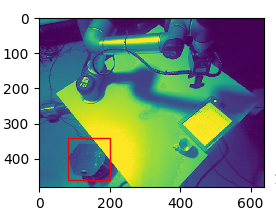
\includegraphics{./images/tb1.png}
\end{minipage}\hfill
\begin{minipage}[t]{.3\textwidth}
\centering
\vspace{0pt}
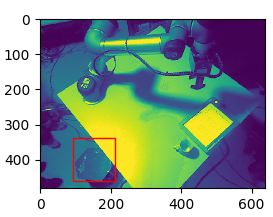
\includegraphics{./images/tb2.png}
\end{minipage}\hfill
\begin{minipage}[t]{.3\textwidth}
\centering
\vspace{0pt}
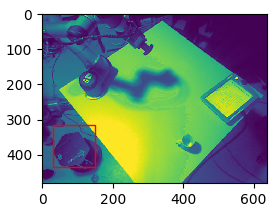
\includegraphics{./images/tb3.png}
\end{minipage}\hfill
\caption{Erkennung des Turtlebots}
\end{figure}
Der Vorteil des verwendeten Ansatzes besteht darin, dass die Erkennung des Turtlebots immer erfolgreich realisiert wird, wenn es komplett in der Szene vorkommt. Wenn aber nur ein Schnitt des Turtlebots sichtbar ist, kann es zu fehlerhaften oder ungenauen Erkennungen kommen. Dies kann verbessert werden, indem die Kamera einen größeren Bereich in Betracht zieht oder indem sie in einer anderen Position steht. Das war aber nicht möglich, weil die Hauptaufgabe der Kinect hieß, die Tasse zu erkennen.

Es ist von Nachteil, dass der Training-Datensatz unterschiedliche Lichtbedingungen nicht berücksichtigte, was die Erkennung des Turtlebots beispielsweise während der Live-Demo negativ beeinflusste. Um dies zu kompensieren, könnte eine Komponente implementiert werden, die vor der Erkennung ein Fine-Tuning des Models anhand von Szenen der neuen Umgebung realisiert, um das Model zur neuen Umständen zu adaptieren.

Darüber hinaus dauerte die Inferenz bei der Erkennung im Durchschnitt 15 Sekunden im Shuttle. Dies wurde mittels eines Parallelisierungsverfahren umgangen, was zur Folge hatte, die Inferenzzeit um 10 Sekunden (ca. 5 Sekunden/Inferenz) im Durchschnitt zu sinken.